\documentclass[sigconf]{acmart}

% --- no ACM copyright block, conference banner or "ACM Reference Format" box (class report) ---
\setcopyright{none}
\settopmatter{printacmref=false}
\renewcommand\footnotetextcopyrightpermission[1]{}
\acmConference{}{}{}
\acmDOI{}
\acmISBN{}
\pagestyle{plain}

% Citations are numbered by default. For author-year citations, uncomment:
% \citestyle{acmauthoryear}
\setlength{\parskip}{0.5\baselineskip}
\begin{document}

\title{Disclosure Without Inference: LLM Agents Anchor on Disclosed Trade Data When Bargaining}

\author{Joey Poh}
\affiliation{%
  \institution{National University of Singapore}
}

\begin{abstract}
With the rapid improvement of LLM capabilities, an agentic economy, where autonomous AI agents act as independent actors that negotiate and settle transactions on behalf of humans, is becoming a reality. AGI Institutions has raised concerns over negotiations across a capability gap~\cite{agiinstitutions2026negotiation}.
Currently, asymmetric capabilities between negotiators are tolerated because the gap is bounded. However, in an agentic economy, asymmetric capabilities could potentially be much more extreme than the human case of a skilled negotiator versus an unskilled one, making it harder to find protocols that work for all parties. One design choice for such a negotiation is a floor mechanism. This is already seen in traditional financial markets: when the Financial Industry Regulatory Authority (FINRA) began publishing US corporate bond trades, investors negotiated better prices and their trading costs fell~\cite{goldstein2007transparency}. This paper investigates whether similar information would be effective for LLM agents.
\end{abstract}

\maketitle

% ======================================================================
\section{Introduction}

The experiment is a dyadic negotiation, where a client agent buys an off-the-run US Treasury note from a single dealer with a private cost. In some conditions, it also sees a summary of other dealers' reported purchases. We build a calibrated bargaining game with a Bayesian benchmark, under which the disclosure raises the client's share by 11\% of the surplus on our test scenarios. We then test a 35B open-weight model that crosses disclosure with belief elicitation.

Disclosure did not reliably improve the LLM's outcome ($-7.3$ percentage points, 95\% CI [$-19.0$, $3.8$]), well short of the Bayesian gain. The client did respond to the disclosure, but by bidding the numbers it was given: its counteroffers moved towards the disclosed typical cost and often sat on the bottom of the disclosed range, where most were rejected. Its stated beliefs did little to drive its actions. In conclusion, an information floor cannot substitute for inference the agent does not perform.

% ======================================================================
\section{Background}

\paragraph{Bargaining with private values.}
When both sides of a trade hold private values, no bargaining procedure can guarantee that every worthwhile trade happens while giving both sides an incentive to be truthful~\cite{myerson1983efficient}. How the surplus is split then depends on the protocol and on what each side knows. Information design studies how a third party can change outcomes by choosing what to reveal~\cite{kamenica2011bayesian}. In corporate bonds, the introduction of trade reporting through TRACE lowered investors' trading costs~\cite{bessembinder2006market,edwards2007corporate}. Those studies measure market-wide averages, whereas we look inside a single negotiation.

\paragraph{LLM agents in bargaining.}
\citet{lewis2017deal} trained negotiation agents end to end. \citet{qian2026strategic} compared humans, LLMs and Bayesian agents in a multi-player trading game and found that similar surplus can hide different strategies: LLMs made concessionary offers that were usually accepted. Like them, we use induced values and a computed benchmark, but we hold the agent fixed and vary its information.

\paragraph{Bayesian theory of mind and anchoring.}
Inferring another agent's private state from its actions can be modelled as Bayesian inverse planning~\cite{baker2017rational,zhixuan2020online}. A client able to read a dealer's cost from its quote would need no disclosure. People, by contrast, often anchor on salient numbers~\cite{tversky1974judgment}, and LLMs show similar biases~\cite{jones2022capturing}. Our design distinguishes Bayesian use of a disclosure from anchoring on it.

% ======================================================================
\section{Bargaining Game with a Bayesian Benchmark}

In this game, a client buys \$10M of an off-the-run 10-year note from one dealer in a game limited to three moves (Figure~\ref{fig:setup}). First, the dealer quotes a price $p$. The client either accepts $p$, or makes a counter-offer $q < p$. The dealer accepts $q$ if and only if $q \ge c$, its private cost.  \begin{figure*}[t]   \centering   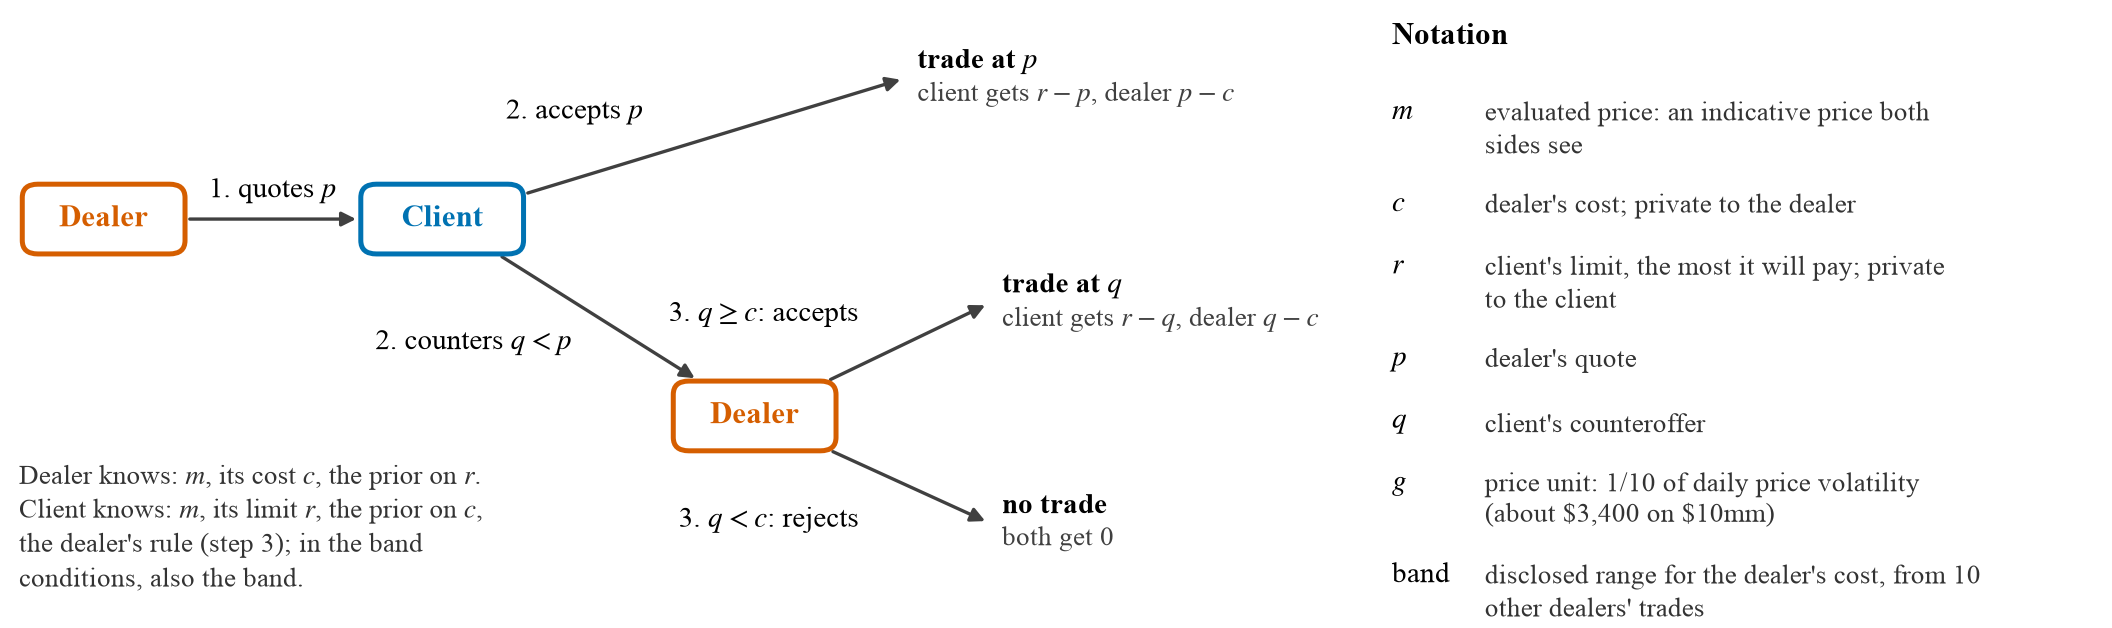
\includegraphics[width=\textwidth]{figures/fig1_setup.png}   \caption{The bargaining game. The dealer quotes a price $p$; the client accepts it or counters with a lower price $q$; the dealer accepts the counter only if it covers its cost $c$, and its decision is final. A trade at price $x$ pays the client $r - x$ and the dealer $x - c$; no trade pays both zero. Each side knows its own private value ($c$ or $r$) and only the distribution of the other's. In the band conditions the client also sees the band.}   \label{fig:setup} \end{figure*}

The client has a private limit $r$, the most it will pay, and earns $r$ minus the price, or zero if there is no trade. Both sides see an indicative evaluated price $m$. Our primary outcome is the client's share of the surplus, zero if there is no trade, or its capture as defined as follows:
\begin{equation}
  \text{Capture} = \frac{r - \text{price}}{r - c}.
\end{equation}

\paragraph{Calibration.}
Each scenario draws the dealer's cost $c$ below $m$ and the client's limit $r$ above it, each at a random distance (LogNormal, median $1g$). Both sides know these distributions. The unit $g$, about \$3{,}400 on \$10mm, is one tenth of the note's daily price volatility, which puts it within the range of real dealer margins.

\paragraph{Disclosure.}
Ten other dealers' reported purchases are centred on the market-wide typical cost, from which this dealer deviates by a random amount $d \sim \mathcal{N}\!\left(0, (0.25g)^2\right)$. In the simulations where the band was disclosed, the client reads:

\begin{quote}
``Reported purchases by other dealers of similar off-the-run notes yesterday (10 trades) averaged $X$ below their evaluated prices. Applied to today's evaluated price, that implies a typical dealer cost of \textit{avg}. Individual dealers' costs vary around the typical level, so this dealer's own cost is within [\textit{low}, \textit{high}] about two times in three.''
\end{quote}

The band's centre is an unbiased but noisy reading of this dealer's cost, with standard deviation $s = 0.356g$, against a prior standard deviation of $0.604g$. The stated range, $\textit{avg} \pm s$, contains the true cost 68\% of the time, so the statement is exactly true.

\paragraph{Rational Client.}
As a benchmark, we compute the play of a Bayesian client. Suppose the client holds a belief $G(q)$, the probability that the dealer's cost is at or below $q$. Then its best counter $q^*$ is the counter that maximises $(r - q)\,G(q)$, and the highest quote it should accept is $\theta = r - \max_q\,(r - q)\,G(q)$. It accepts the quote $p$ if $p \le \theta$, and otherwise counters at $q^*$: a lower counter means a better price but a higher chance of rejection. Without the band, $G$ is the prior. With the band, $G$ is the Bayesian posterior.

\paragraph{The Dealer.}
The same fixed algorithm in every condition. It chooses the quote that maximises its expected profit over the prior on the client's limit, assuming an uninformed client. It rounds the quote to 0.001 points, and accepts any counter at or above its cost. It quotes $m - 0.425g$ in 88\% of scenarios, so its quote reveals little about its cost: the quote explains 18\% of the variation in the cost.

\paragraph{Value of disclosure.}
We play the rational client against this dealer at the true cost and limit. Over 1{,}000 scenarios, the band raises the client's surplus by 11.35\% of the total surplus. On our 50 test scenarios it raises capture from 0.621 to 0.732 ($+0.111$). This is the most a client that uses the band perfectly can gain. It is each side's best response to its stated beliefs, not an equilibrium.

% ======================================================================
\section{Experiments}

\subsection{Design}

\paragraph{Choosing the client.}
Before the experiment, we chose the client model with a short pilot on separate scenarios. The pilot checked basic competence, for example, that at least 90\% of the model's counteroffers were below the quote and within its own limit. Our first choice, Qwen3.6-35B, failed this check (67\%). Ornith-1.5-35B passed (92\%) and was used throughout. It runs at temperature 0.5 with reasoning off, so it must bargain without step-by-step working.
\paragraph{The Experiment.}
We varied two things: whether the client sees the band, and whether we elicit its beliefs. Belief elicitation asks for the client's probability that the dealer's cost lies below each of nine prices, once before it sees the quote and once after, so that we can compare its beliefs with a Bayesian client's. Each condition was played on the same 50 scenarios, twice each. The main test (the band raises the client's capture without belief elicitation) and its decision rule were pre-registered before any negotiation with the band. All confidence intervals are 95\% bootstrap intervals over scenarios (10,000 resamples).

% ----------------------------------------------------------------------
\subsection{LLM Agent Bargaining Results without Disclosure}

Without the band, the client almost always made a counteroffer (98--99\% of negotiations), while a rational client would usually accept the quote. Its counteroffers were also low: on average $1.3g$ below the evaluated price. About half were rejected, so the client kept only 36--41\% of the surplus. A rational client keeps 62\%.


The client's counteroffers sit on numbers it has been given. Without belief elicitation, 77 of its 98 counteroffers land on one of two prices from the briefing: the typical dealer cost, $1g$ below the evaluated price (about \$3,400 on the \$10mm trade; 46 counteroffers), or the low end of the briefing's 80\% range of costs, $1.9g$ below (31 counteroffers; Figure~\ref{fig:counters}a). Belief elicitation itself also supplied prices to bid. It asks for the probability that the dealer's cost is below each of nine listed prices, and with elicitation, half of the client's counteroffers sat exactly on one of them ($1.25g$, $1.5g$ or $2g$ below the evaluated price). Without elicitation, the client almost never bid these prices.


Its stated beliefs do not drive its bids. Its beliefs imply a counteroffer about $0.47g$ below the evaluated price, but they do not predict its actual counteroffers (rank correlation $0.08$). Nor do its counteroffers rise with its own limit.

% ----------------------------------------------------------------------
\subsection{Evaluating if an Information Floor Helps}

The band did not improve the LLM client's outcome. Without belief elicitation, the client kept 41\% of the surplus without the band and 33\% with it (Figure~\ref{fig:capture}). The difference, $-7.3$ percentage points (95\% CI [$-19.0$, $3.8$]), is not significant, so our pre-registered main test is not supported. A rational client facing the same dealer raises its share from 62\% to 73\% with the band, a gain of 11 percentage points. That gain lies above the LLM's entire confidence interval. So, even at best, the LLM gained about a third of what the band offers. With belief elicitation, the band made no difference either ($-0.2$ points, 95\% CI [$-10.2$, $9.7$]).


\begin{figure}[t]
  \centering
  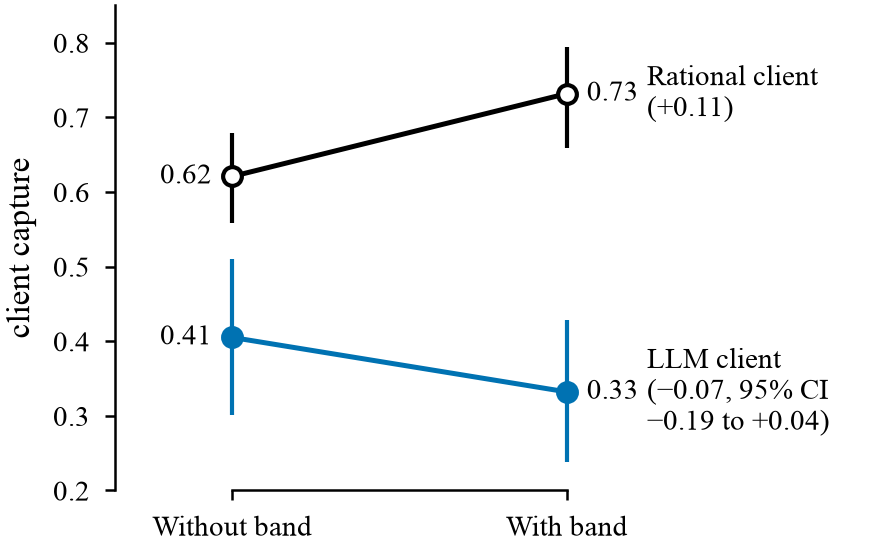
\includegraphics[width=0.85\columnwidth]{figures/fig2_results.png}
  \caption{Client capture without and with the band. Rational client: open markers; LLM client, without belief elicitation: filled markers. The band raises the rational client's capture by 11\% of the surplus; the LLM's change is not significant.}
  \label{fig:capture}
\end{figure}

% ----------------------------------------------------------------------
\subsection{How the LLM Agent Used the Band}

The LLM agent reacted to the band, but by bidding its numbers rather than reasoning with them. As predicted, its counteroffers moved towards the band's centre, by $0.16g$ without belief elicitation (95\% CI [$0.08$, $0.24$]) and $0.26g$ with it ([$0.19$, $0.33$]).

An exploratory look in Figure~\ref{fig:counters} shows this. Without belief elicitation, 26\% of counteroffers sat exactly on the bottom of the band's stated range, against 1\% without the band. The dealer's cost lies below that point only about 16\% of the time, so 77\% of these counteroffers were rejected, which explains why the estimated effect of the band is negative. The band did not replace the briefing's numbers: the typical cost from the briefing was still the client's most common counteroffer. And, as without the band, its counteroffers did not depend on its own limit, although a rational client with a higher limit bids higher to make a rejection less likely.

\begin{figure}[t]
  \centering
  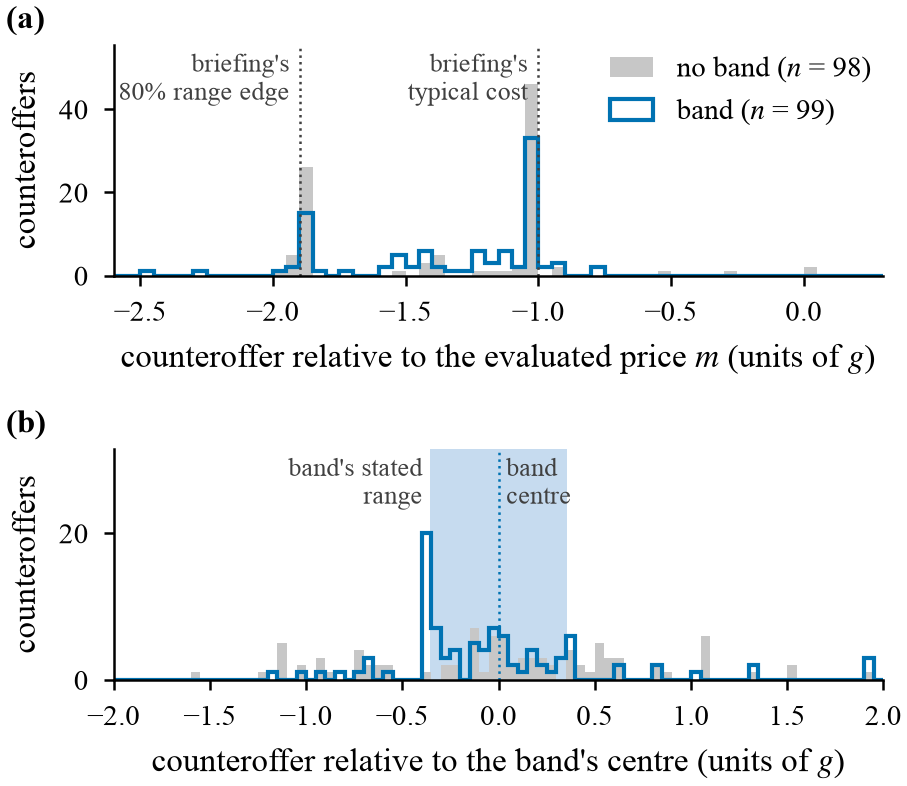
\includegraphics[width=\columnwidth]{figures/fig3_counters.png}
  \caption{Where the client bids, without belief elicitation. (a)~Without the band (grey), counteroffers pile up on numbers in the briefing. (b)~With the band (blue), they move onto the band's own numbers, most often the bottom of its stated range (shaded).}
  \label{fig:counters}
\end{figure}


\subsection{What the LLM Agent Believed}
Belief elicitation shows that the band changed what the client believed, but less than it should have, and that the client acted on its beliefs only weakly. With the band, the client's best guess of the dealer's cost moved $0.23g$ towards the band's centre (95\% CI [$0.14$, $0.34$]), about half as far as a Bayesian client's ($0.46g$; Figure~\ref{fig:beliefs}a). Its best guess also moved $0.16g$ closer to the true cost (95\% CI [$0.07$, $0.27$]), again about half the Bayesian gain (Figure~\ref{fig:beliefs}b; this comparison is exploratory). Its belief as a whole, however, was no closer to the Bayesian belief with the band than without it (change in mean squared error $+0.012$, 95\% CI [$-0.004$, $0.030$]). Most importantly, its counteroffers followed its beliefs only weakly. Without the band, the counteroffers its stated beliefs imply did not predict the ones it made (rank correlation $0.08$). With the band they did, modestly ($0.31$), but partly because the band pulled beliefs and bids towards the same number; removing that common pull leaves $0.22$ (exploratory).

The client also did not weigh evidence by how informative it was. After seeing the dealer's quote, which reveals little about the cost, it concluded that the cost was higher, yet it moved only partly towards the band, which is far more informative. The LLM noticed the band, but did not weigh it correctly, and its bids followed its beliefs only weakly.

\begin{figure}[t]
  \centering
  \includegraphics[width=\columnwidth]{figures/fig4_belief_shift.png}
  \caption{How far the band moves the client's best guess of the dealer's cost (the median of its stated belief, before the quote), in the conditions with belief elicitation. (a)~Distance from the best guess to the band's centre. (b)~Distance from the best guess to the true cost. Lower is closer. The LLM's guess moves the right way, but about half as far as a Bayesian client's. Mean over 50 scenarios with 95\% CIs.}
  \label{fig:beliefs}
\end{figure}


% ----------------------------------------------------------------------
\subsection{Confirmation from Unseen Scenarios}

We repeated the experiment on 20 never-seen scenarios. Figure~\ref{fig:heldout} compares the two and confirms that the two main findings hold. First, the band again had no reliable effect on the client's share of the surplus. Disclosure is worth little on the new scenarios, so they cannot show whether the LLM falls short of the rational gain. Second, in Figure~\ref{fig:heldout}b, the client again moved its bids towards the band's centre, confirming that the LLM agent anchors on the numbers given.

We also asked whether the band changes what the client believes about the dealer's cost (Figure~\ref{fig:heldout}c). In the main experiment, the client's belief followed the band's centre about a third as closely as a Bayesian client's (slope 0.31 against 0.84); on the new scenarios it did not follow it at all (slope 0.00). The band reliably changed where the client bid, but its effect on what the client believed was weak and did not replicate.

\begin{figure}[t]
  \centering
  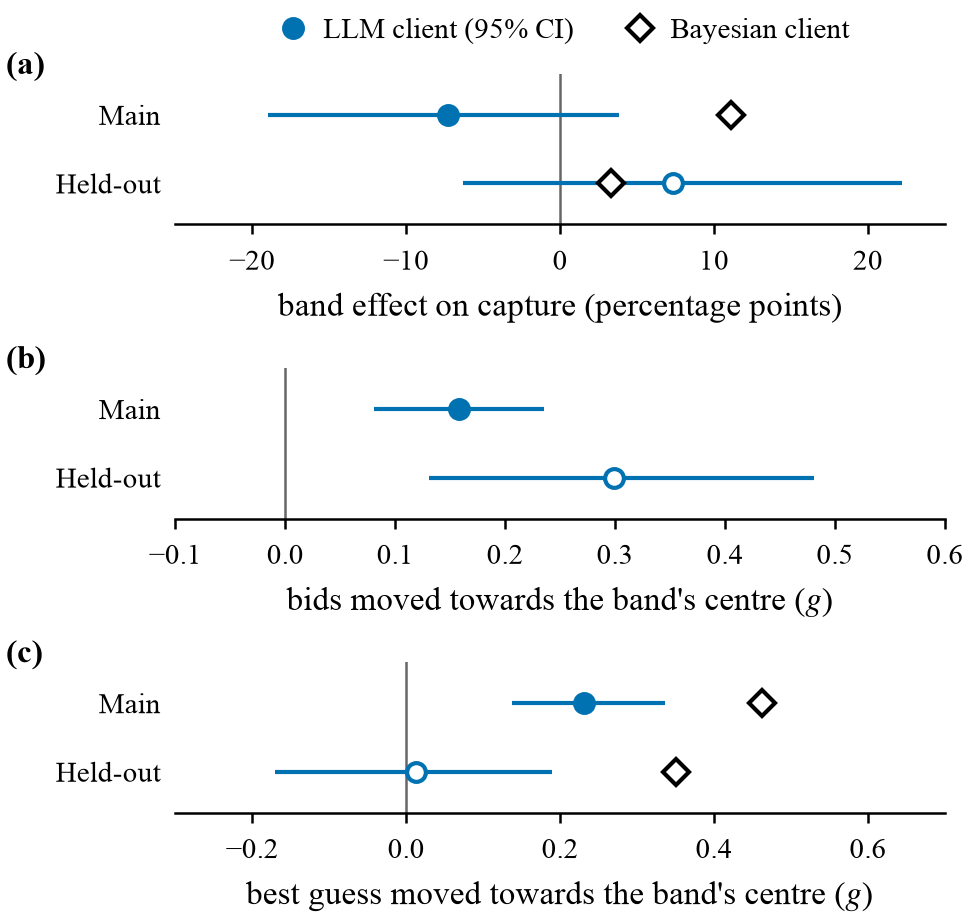
\includegraphics[width=\columnwidth]{figures/fig5_heldout.png}
  \caption{Main experiment (filled; 50 scenarios, two runs) against 20 held-out scenarios (open; one run), with 95\% CIs. Diamonds: rational or Bayesian client. (a)~The band's effect on capture. (b)~How far bids moved towards the band's centre. (c)~How closely the client's belief follows the band's centre (slope).}
  \label{fig:heldout}
\end{figure}

% ======================================================================
\section{Limitations and Future Work}

This experiment was deliberately simple, so future work should test whether the failure is specific to this setup. First, every client is told the distribution of dealers' costs, as parity with the rational client requires, but the briefing states it as concrete prices, and these became the client's most common bids. Stating the same distribution without prices would show whether the anchoring depends on being given a price. Second, the client ran with reasoning off, to model a capability-bounded agent; repeating the experiment with reasoning on would show whether step-by-step working lets it use the band. Third, varying the prompt's wording would show whether the anchoring is robust or tied to how the numbers are presented. Finally, testing other model families and sizes would show whether any LLM agent can use an information floor to close a capability gap.

% ======================================================================

% ======================================================================
\section{Conclusion}

The information floor (disclosing other dealers' trade data) did not reliably improve an LLM client's outcome. It delivered significantly less than a Bayesian client gains from the same information. While the client did not ignore the disclosure, it treated the disclosed numbers as prices to bid. These results suggest Ornith-1.5-35B does not have the inference needed to use it. Hence, an agent's fundamental capability remains the most important factor. Given that the LLM agent is anchored on the given numbers, how the information is published is perhaps of the same importance as whether to publish. Asking an agent about its beliefs is not neutral either. The prices in our elicitation questions became anchors, and the agent's stated beliefs were at best weakly related to how it bid.


% ======================================================================
\bibliographystyle{ACM-Reference-Format}
\bibliography{refs}

\end{document}
